\section{Introduction}

% \blue{Shall we talk about the shared spectrum, like in the IPSN and WoWMoM paper? Prof. Mark in the author list?}


Quantum sensors, being strongly sensitive to external disturbances, are able to measure various physical phenomena with extreme sensitivity.
These quantum sensors interact with the environment and have the environment phenomenon or parameters encoded in their state~\cite{RevModPhys.quantumsensing}.
A group of distributed quantum sensors, if prepared in an appropriate entangled state, can further enhance the estimation of a single continuous parameter, improving the standard deviation of measurement by a factor of $1/\sqrt{N}$ for $N$ sensors~\cite{Giovannetti_2011}.
Recently, experimental physicists successfully demonstrated a reconfigurable entangled radio-frequency photonic sensor network~\cite{PRL20-qsn,arizona21-thesis}.
The experiments establish a connection between the entanglement structure and the achievable quantum advantage in different distributed sensing problems.

In the classical world, a network of wireless sensors is well-known to facilitate spatially distributed sensing.
For example, in the task of indoor RF localization, a transmitter signal's angle-of-arrival observed from different locations facilitates localization via triangulation~\cite{nsdi13-arraytrack}.
RF localization is a key technology for location-based services.
An improvement in RF localization will be very beneficial to an array of mobile applications and thus generate huge economic effects.
For example, getting a fine-grained location in supermarkets, libraries, or museums will be very useful.
Precise location is very important in augmented reality applications.
For outdoor spectrum patrolling, we may want to detect and locate the intruders that illegally use unauthorized spectrum~\cite{infocom18-spectrum}.



\begin{figure*}[t]
    \centering
    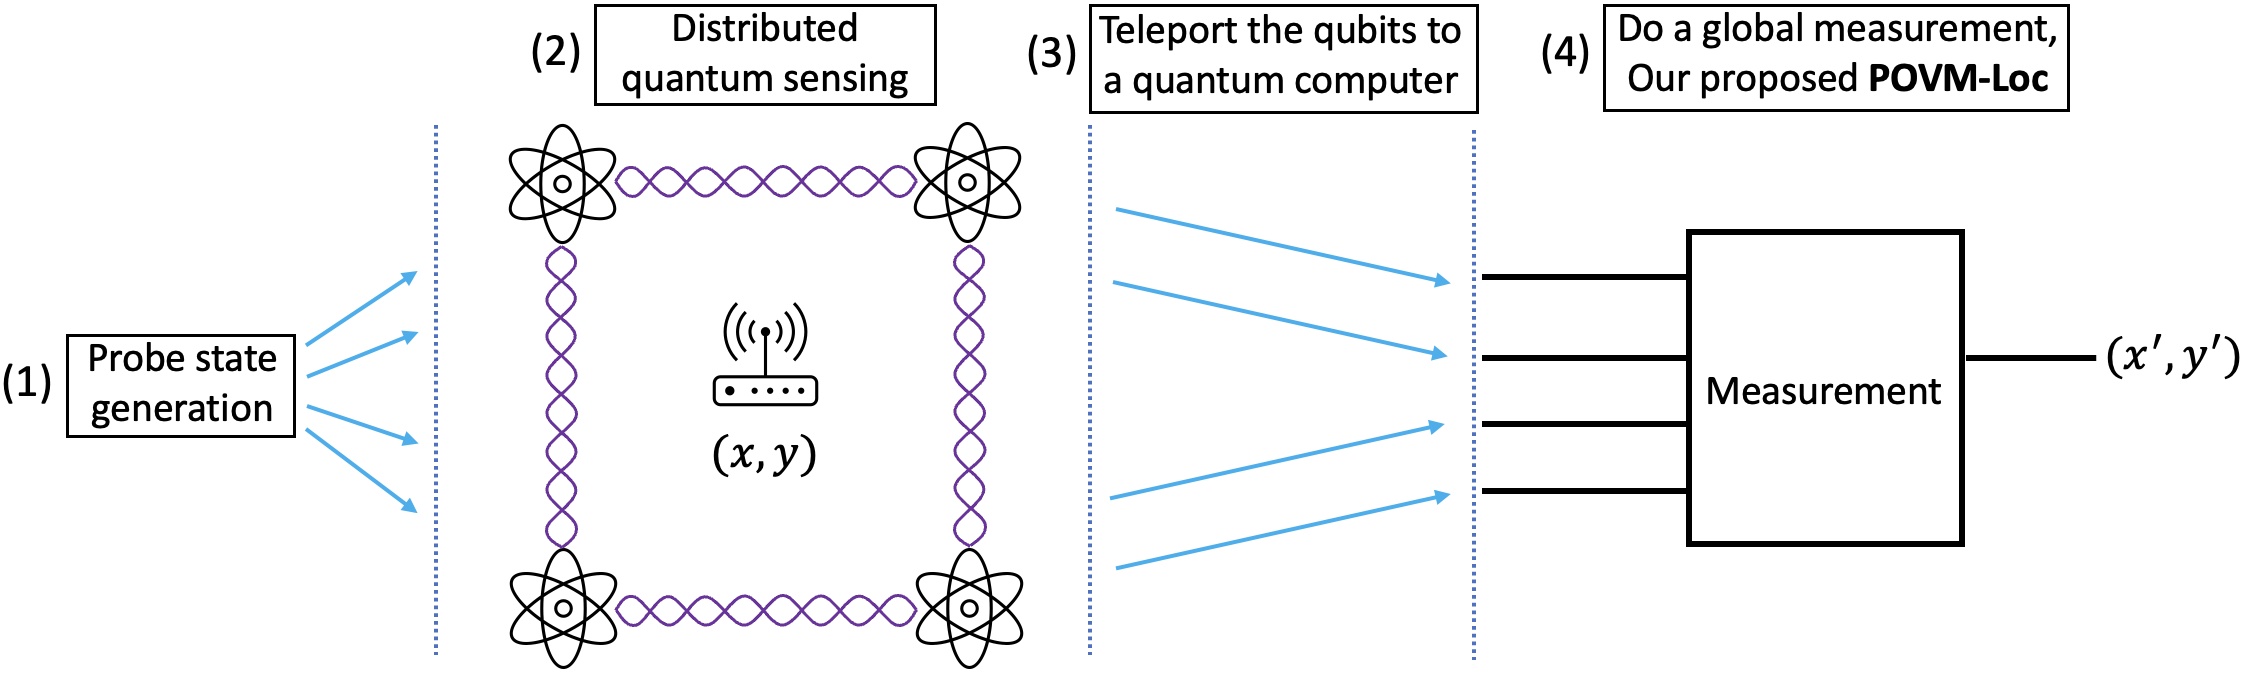
\includegraphics[width=0.98\textwidth]{chapters/icc/figures/overall.png}
    % \vspace{-0.1in}
    \caption{Overall architecture of localizing an RF transmitter in a quantum sensor network.}
    % \vspace{-0.1in}
    \label{fig:quantumoverall}
\end{figure*}


\eat{Quantum sensors vs classical sensors ?:
1) Each quantum sensor is very precise. 2) Square root N factor. 3) First step. Starting a field.
}

\para{Motivation for Quantum Sensors.}
Albeit classical sensors are omnipresent, there are big motivations to explore quantum sensors.
Quantum sensing is an emerging field that leverages the quantum properties of light and matter at atomic/subatomic scales and has the potential to sense signals at an unprecedented level of precision.
For example, physicists in the year 2016 used squeezed quantum states to improve the sensitivity of the Laser Interferometer Gravitational-wave Observatory (LIGO) detector and successfully detected gravitational waves.
In~\cite{PRL20-qsn}, researchers use some distributed quantum RF-photonic sensors to estimate the amplitude and phase of a radio signal.
They showed the performance of sensing a global property of the RF wave is enhanced by leveraging a shared multipartite entangled state produced by squeezed light.
In their experiments, the estimation variance of RF amplitude and phase both beat the standard quantum limit by over 3 dB.
The precision improvement factor of $1/\sqrt{N}$ for $N$ sensors is known as reaching the Heisenberg limit.
Motivated by the above, we aim to leverage quantum sensors to perform some canonical tasks and thus open a new avenue of research.

\eat{In principle, merely replacing the classical sensors with quantum RF-photonic sensors and using the same classical localization algorithms will lead to accuracy improvement, since the estimation of RF amplitude and phase is more accurate.
In this scenario, the quantum measurement happens at individual sensors.
For the RF-photonic sensors, the quantum measurement is the homodyne measurement.
The individual sensors will post-process the measurement data and get more accurate classical data (amplitude, phase, RSS), thus, leading to more accurate localization.}

\para{Quantum localization on quantum data.}
The canonical task we picked is RF transmitter localization~\cite{nsdi13-arraytrack,pmc22-deepmtlpro}.
We pose the localization problem as a quantum state discrimination problem~\cite{bergou-review-2007}. 
The overall architecture is illustrated in Fig.~\ref{fig:quantumoverall}.
First, a probe state is generated and distributed to a network of quantum sensors.
Second, the quantum sensors make interactions with the signal sent from a transmitter. 
The location of the transmitter is encoded in the quantum state at the quantum sensors.
Third, the quantum states will be teleported~\cite{ton22-quantum} to a centralized node.
Finally, at the central node, we consider global measurement where all the teleported qubits are measured simultaneously. 
The measurement outcome indicates the location of the transmitter.
Quantum measurement via positive operator-valued measure (POVM) is the core part of quantum state discrimination.
POVM is the general quantum measurement defined as a set of positive semi-definite Hermitian matrices $\{E_i\}$ and each Hermitian matrix $E_i$ is associated with the measurement outcome $i$~\cite{qcqi-book}.
In our context, we further associate an outcome $i$ to a two-dimensional location $(x, y)$.
Thus, we discriminate the quantum state via POVM and the POVM's output indicates the transmitter location.


\para{Contributions.} 
To the best of our knowledge, we are the first to explore using a distributed set of quantum sensors to localize an RF transmitter via a quantum localization approach. 
Our implementation is open source at \footnote{\url{https://github.com/caitaozhan/QuantumLocalization}}.
In this context, we make the following three contributions.
\begin{enumerate}
    \item Mathematically models a quantum sensor and introduces the problem of transmitter localization via a quantum sensor network. Section~\ref{sec:quantum_problem}.
    \item Design and implement \povm and its improved version \povmpro, two quantum localization methods using a quantum sensor network. Section~\ref{sec:povm}.
    \item Evaluate our techniques via simulations and demonstrate the effectiveness of our developed techniques. Section~\ref{sec:quantum_eval}.
\end{enumerate}
